
\chapter{Aspekt bezpieczeństwa w systemach rekomendacyjnych}
Systemy rekomendacyjne muszą gromadzić wiele danych o użytkownikach w celu wykonania trafnego przewidywania potencjalnych obiektów zainteresowania. W zależności od metody serwis dokonuje porównania  profili użytkowników, oblicza podobieństwo pomiędzy użytkownikami czy grupuje użytkowników o zbliżonych cechach. Gromadzone w tym celu dane mogą pozwolić na identyfikacje użytkownika przez co twórcy systemu muszą wybierać pomiędzy prywatnością użytkowników, a skutecznością w dokonywaniu rekomendacji. Taki system z wrażliwymi danymi użytkowników może stać się celem grup hakerskich chcących pozyskać tak cenne informacje. Stąd zapewnienie bezpieczeństwa podczas przesyłania danych pomiędzy serwisami oraz dokonywania obliczeń na nich powinno stać się priorytetem. Jednak większość prac skupia się na zwiększeniu skuteczności czy wydajności \cite{recent_developments}.

\section{Prywatność}
Prywatność w kontekście systemów rekomendacyjnych oznacza, że podczas pracy systemy żadne dane nie mogą wyciec, a także otrzymana predykcja nie powinna pozwolić na identyfikację użytkownika. Na rysunku \ref{fig:podatnosci} przedstawiono potencjalne miejsca, w których dane mogą zostać przechwycone. Jak widać atakujący mogą uzyskać dane podczas wprowadzania ich do systemu, przesyłania ich pomiędzy poszczególnymi komponentami usługi, jak i w trakcie wysłania predykcji do użytkownika. Idealny, zachowujący prywatność system rekomendacyjny powinien być bezpieczny bez znaczącej utraty na wydajności jako całości, a przede wszystkim bez zmniejszenia trafności rekomendacji. 
    Y = X + C, gdzie C jest szumem dodanym do oryginalnej macierzy X. W praktyce każdy wiersz C generowany jest niezależnie,
\begin{itemize}
    \item perturbacja danych (ang. \textit{data perturbation}),
    \item bezpieczne obliczanie wieloczęściowe (ang. \textit{secure multiparty computation}).
\end{itemize}

\begin{figure}
    \centering
    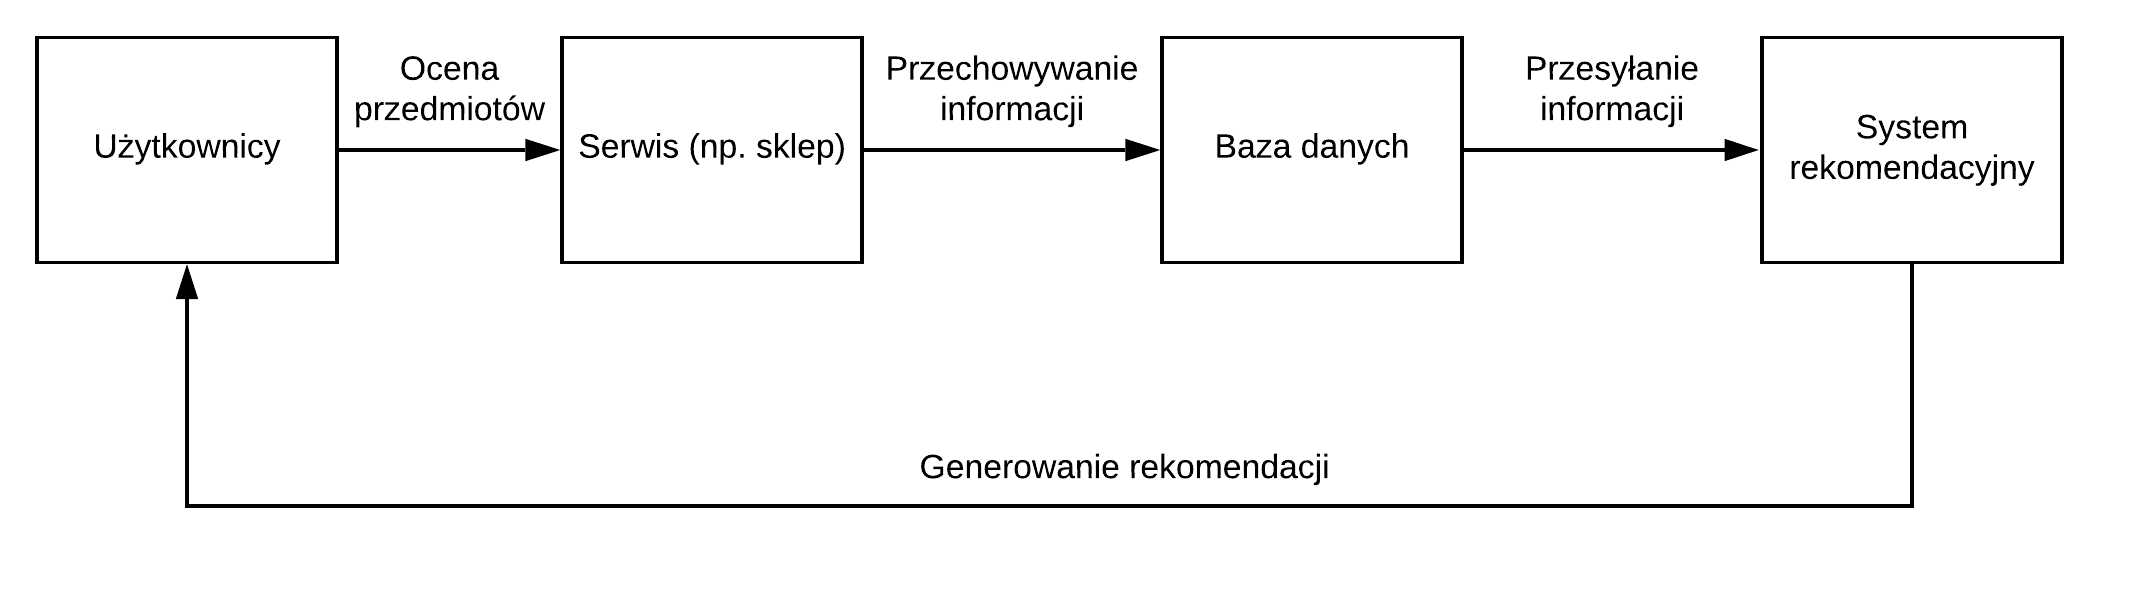
\includegraphics[scale=0.85]{images/podatnosci.png}
    \caption{Potencjalne podatności systemu.}    Źródło: opracowanie własne na podstawie \cite{practicalPrivacy}

    \label{fig:podatnosci}
\end{figure}
\section{Perturbacja danych}
Właściciel danych (użytkownik) dokonuje perturbacji własnych danych, a następnie przesyła je w celu dalszego przetwarzania.
Wyróżniamy następujące rodzaje perturbacji danych:
\begin{itemize}
    \item addytywne - opisane następującym wzorem 
    Y = X + C, gdzie C jest szumem dodanym do oryginalnej macierzy X. W praktyce każdy wiersz C generowany jest niezależnie,
    \item multiplikatywne - opisane wzorem Y = MX, gdzie M jest to macierz przez którą przekształcana są dane źródłowe. W przypadku tej metody nie ma gwarancji, że zostanie zachowana prywatność (przypadek w którym atakujący zna porcję danych w zbiorze X oraz ich odpowiednik w zbiorze M),
    \item prywatność różnicowa - wyróżnia się trzy podejścia w zależności od momentu wprowadzenia szumu: do danych wejściowych, w trakcie przetwarzania lub do danych wyjściowych.
\end{itemize}

Głównym problemem w wykorzystaniu perturbacji danych w celu zapewnienia prywatności jest brak gwarancji, że uzyskane wyniki będą tak samo trafne jak w przypadku bez wprowadzenia szumu w danych.

\section{Bezpieczne obliczanie wieloczęściowe}

Metoda pozwala rozproszonym stronom na wspólne obliczanie bez konieczności odkrywania ich prywatnych danych wejściowych oraz wyjściowych. Ponadto zastosowania obliczania wieloczęściowego nie wymaga użycia zaufanej trzeciej strony (bezpieczeństwo pozostaje takie samo jak w przypadku wykorzystania trzeciej strony). 
Wyróżniane są następujące rozwiązania:
\begin{itemize}
    \item rozwiązania oparte na bezpiecznym dodawaniu wektorów (\textit{ang. Secure Vector Addition based Solutions}),
    \item szyfrowanie homomorficzne,
    \item podejścia oparte na bezpiecznych produktach skalarnych (\textit{ang. Secure scalar product based approach}),
    \item podejścia oparte o "zniekształcony obwód" (\textit{ang. Garbled circuit based approach}).
\end{itemize}

Jednak bezpieczne obliczanie wieloczęściowe nie sprawdza się w komercyjnych rozwiązaniach opartych o rekomendacje. Spowodowane jest tym, że metoda ta na ten moment nie może być rozpatrywana przy systemach wymagających działania w czasie rzeczywistym. \cite{secureMultipartyComputation}
